\documentclass{sosg-informe}

\usepackage{tikz}
\usetikzlibrary{positioning,arrows.meta}

\graphicspath{{../../geodatos/estudios/santa-cruz/figuras/}{figuras/}}

\title{Nivel preliminar de inundación por lluvia medida:\\la regla v0.2 de la alerta de SOS Galápagos}
\titulocorto{Nivel preliminar de inundación (regla v0.2)}
\numero{2026-07}
\estado{Borrador para discusión}
\titulocita{Nivel preliminar de inundación por lluvia medida: la regla v0.2 de la alerta de SOS Galápagos}
\relacionados{Issues \issue{30}, \issue{52}, \issue{62} y \issue{80} · repositorio mayait/sosgalapagos-datos}
\date{4 de noviembre de 2026}

\begin{document}
\maketitle

\begin{abstract}
Desde el 2 de noviembre de 2026, el panel de clima de SOS Galápagos muestra para cada zona poblada un nivel preliminar de inundación (bajo, medio, alto o muy alto) calculado cada 5 minutos con la lluvia que miden los pluviómetros de IERSE, INAMHI y USFQ GSC. Este informe describe la regla que lo produce, la versión 0.2. La lluvia de referencia de una zona es el máximo, entre sus estaciones válidas, de la lluvia ponderada en ventanas móviles de 1, 3 y 24~h. Basta que una ventana supere su umbral: 30, 60 o 100~mm para el nivel \alto. Los umbrales bajan un 20\,\% con suelo húmedo, según los cortes de humedad antecedente del SCS (36 y 53~mm en 5 días). El nivel se mantiene 8~h. Si las estaciones callan durante una alerta, el nivel sube a \enquote{muy alto}, y si no hay datos válidos se informa \enquote{sin datos}, nunca \enquote{bajo}. La regla es juicio experto calibrado con un solo evento, el del 30 de octubre de 2026 en La Cascada (Puerto Ayora), y su probabilidad es cualitativa. Se reprodujo con el mismo código del recolector sobre la lluvia archivada desde abril de 2026. El 30-oct, la regla habría dado \alto{} en La Cascada a las 15:50 y \enquote{muy alto} a las 20:35. El primer aviso lo provocó Santa Rosa, una estación que no drena hacia La Cascada, una hora antes de que el modelo hidrológico llene el vaso. En seis meses de registro, fuera del 30-oct, la regla dio \alto{} en La Cascada un solo día (4-oct), por la ventana de 24~h, con lluvia poco intensa. La evaluación con 500 tormentas sintéticas por isla está en el Informe técnico 2026-02.
\palabrasclave{alerta temprana; inundación repentina; umbrales de lluvia; humedad antecedente; pluviómetros; prueba retrospectiva; Galápagos.}
\end{abstract}

\begin{aviso}
El nivel que describe este informe es \textbf{preliminar, no oficial y de elaboración propia}. No es una alerta de la SNGR, del INAMHI ni del ECU~911. La regla es \textbf{juicio experto calibrado con un solo evento} y su probabilidad es cualitativa: no tiene base estadística. Los tiempos del vaso y del pico en La Cascada salen de \textbf{modelos propios} sin calibrar, no de observaciones. El análisis lo preparó un equipo asistido por agentes de inteligencia artificial, sin visitas de campo ni revisión profesional externa, y no expresa una posición institucional de la USFQ. Usa lluvia medida del IERSE (CC BY-NC-ND 4.0; \citealp{orellana2023}), del INAMHI y del USFQ GSC (licencia por confirmar); los productos derivados de esas series quedan sujetos a sus licencias y al permiso de sus titulares.
\end{aviso}

% =====================================================================
\section{Introducción}

En Santa Cruz y San Cristóbal no hay ríos permanentes: las inundaciones llegan por quebradas secas que se activan con lluvia intensa y responden en minutos u horas. El 30 de octubre de 2026, la red IERSE-WSN midió 61--73~mm en una hora y 179--240~mm en el día en la parte media y alta de Santa Cruz \citep{orellana2023}. Esa noche se inundó el barrio de La Cascada, en Puerto Ayora, y una persona falleció en la cañada El Aguacatal. La red transmitía casi en tiempo real, pero no tenía umbrales, nadie la vigilaba de noche y no estaba conectada a ningún protocolo. Además, dejó de transmitir a las 21:22--21:25, en el peor momento de la tormenta.

A partir de ese evento, SOS Galápagos conectó al recolector de su panel de clima una regla de aviso por lluvia medida: la v0.1 primero y, desde el 2 de noviembre, la v0.2. La revisó el especialista en gestión de riesgos del comité de estudios. La regla convierte la lluvia de los pluviómetros en un nivel preliminar por zona, con un color y una probabilidad cualitativa. Sigue la lógica de los umbrales de lluvia para crecidas repentinas \citep{georgakakos2006,norbiato2008}, pero sin un modelo hidrológico en tiempo real: los umbrales son fijos, salvo un ajuste por humedad del suelo.

Este informe \emph{describe} la regla: sus datos, sus ecuaciones, las decisiones de diseño y su comportamiento con la lluvia medida desde abril de 2026. Para la prueba retrospectiva se usó el mismo código que corre en el servidor. La \emph{evaluación} frente a un conjunto amplio de tormentas está en el Informe técnico 2026-02 \citep{maya2026idf}, que propaga 500 tormentas sintéticas por isla con un modelo 2D; sus resultados se discuten en la sección~\ref{sec:discusion}.

% =====================================================================
\section{Área de estudio y datos}

\subsection{Zonas}
La regla v0.2 define cuatro zonas (tabla~\ref{tab:zonas}). Solo La Cascada tiene una calibración, y con un único evento. Las demás llevan la marca \enquote{sin calibrar} en el panel. Cerro Crocker queda fuera de todas las zonas porque su pluviómetro parece obstruido desde agosto de 2026 (\issue{56}).

\begin{table}[ht]
  \centering\small
  \caption{Zonas de la regla v0.2, estaciones asignadas y peso $w_s$ de cada una (\texttt{clima/recolector/umbrales\_inundacion.json}).}
  \label{tab:zonas}
  \begin{tabularx}{\linewidth}{>{\raggedright\arraybackslash}p{3.3cm}>{\raggedright\arraybackslash}X>{\raggedright\arraybackslash}p{3.6cm}}
    \toprule
    Zona & Estaciones (peso) & Estado \\
    \midrule
    La Cascada (Puerto Ayora) & Los Guayabillos (1); Santa Rosa (0,75); INAMHI M0191 Puerto Ayora (1); estación particular WeatherLink de Puerto Ayora (1) & calibrada con un solo evento (30-oct) \\
    \addlinespace
    Parte alta de Santa Cruz (Bellavista, Santa Rosa) & Santa Rosa (1); Los Guayabillos (1) & sin calibrar; el riesgo principal son los cruces de quebradas con vías \\
    \addlinespace
    San Cristóbal & GSC: El Junco, Cerro Alto, El Mirador y Merceditas (1 cada una); INAMHI M0221 Puerto Baquerizo Moreno (1) & sin calibrar: no hay evento de referencia \\
    \addlinespace
    Isabela (Puerto Villamil) & ninguna & sin estaciones en tiempo real: siempre \enquote{sin datos} \\
    \bottomrule
  \end{tabularx}
\end{table}

El peso de 0,75 de Santa Rosa en La Cascada es el cociente entre la lluvia del día 30-oct en Los Guayabillos y en Santa Rosa ($179/238$). Las dos estaciones útiles están fuera de la cuenca de La Cascada: Los Guayabillos, a 0,4~km de su borde, y Santa Rosa, a 6,6~km, en una vertiente que no drena hacia el barrio. El INAMHI M0191 y la estación particular WeatherLink están en la costa, aguas abajo del vaso.

\subsection{Lluvia medida}
\begin{itemize}
  \item \textbf{IERSE-WSN} (Universidad del Azuay): cuatro estaciones en Santa Cruz, con un registro cada ${\approx}\,5$~min desde abril de 2026 y pluviómetro de balancín de 0,2~mm. Marca la hora de Galápagos (UTC$-6$). Llega al servidor por un puente desde una máquina en Ecuador.
  \item \textbf{INAMHI}: M0191 (Puerto Ayora, a 1,4~km de La Cascada) y M0221 (Puerto Baquerizo Moreno), con lluvia cada 5~min y un historial horario de respaldo que la fuente guarda solo 90 días. Usa la hora continental (UTC$-5$).
  \item \textbf{USFQ GSC}: El Junco, Cerro Alto, El Mirador y Merceditas, en San Cristóbal, cada 5~min. También marca la hora continental, aunque diga \enquote{Z}.
  \item \textbf{Estación particular WeatherLink} (Puerto Ayora, Davis Vantage Vue): balancín de 0,254~mm, que subestima la lluvia intensa. Se descartan los saltos de más de 100~mm/h.
\end{itemize}
El recolector guarda todo en una base SQLite con las horas en UTC; la conversión de husos se hace al leer cada fuente. Los pluviómetros de balancín subestiman la lluvia de más de 50~mm/h. Cuando una estación deja de transmitir, la lluvia de ese tramo no se mide: no queda en cero ni se acumula para después.

\subsection{Referencias hidrológicas de La Cascada}
Los umbrales se apoyan en el estudio preliminar de La Cascada (\texttt{geodatos/estudios/la-cascada/}), que es un \emph{modelo propio sin calibrar}:
\begin{itemize}
  \item cuenca de 42,33~km² que termina en un vaso cerrado de 50\,000--62\,000~m³, sin cauce hasta el mar;
  \item número de curva SCS de 68 en condición normal (47 en seca y 83 en húmeda), con un valor central de 76 \citep{mishra2003};
  \item tiempo de concentración de 1,5--3,5~h según Kirpich y Témez \citep{kirpich1940,temez1978};
  \item el 30-oct, según el hidrograma modelado, el vaso se llenó entre las 16:50 y las 18:10 y el pico llegó entre las 21:40 y las 22:50. El modelo 2D sitúa la llegada de 0,1~m al centro del barrio a las 20:55 \citep{maya2026idf}.
\end{itemize}

% =====================================================================
\section{Métodos}\label{sec:metodos}

La regla se ejecuta en \texttt{clima/recolector/inundacion.py} cada vez que corre el recolector (cada 5~min) y lee sus parámetros de \texttt{umbrales\_inundacion.json}. La figura~\ref{fig:esquema} resume la cadena de cálculo.

\begin{figure}[t]
  \centering
  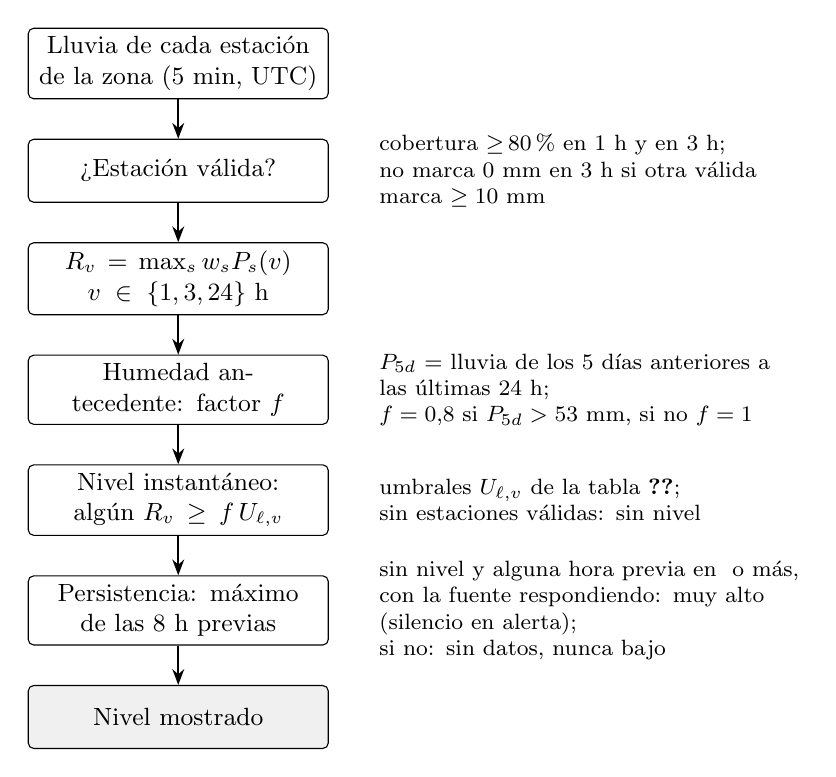
\begin{tikzpicture}[
      font=\small,
      caja/.style={draw, rounded corners=2pt, align=center, minimum height=8mm, text width=3.6cm, inner sep=3pt},
      nota/.style={align=left, text width=5.4cm, font=\footnotesize, inner sep=1pt},
      flecha/.style={-{Stealth[length=2mm]}, thick}]
    \node[caja] (est) {Lluvia de cada estación de la zona (5~min, UTC)};
    \node[caja, below=5mm of est] (val) {¿Estación válida?};
    \node[caja, below=5mm of val] (R) {$R_v = \max_s w_s P_s(v)$\\$v \in \{1, 3, 24\}$~h};
    \node[caja, below=5mm of R] (f) {Humedad antecedente: factor $f$};
    \node[caja, below=5mm of f] (inst) {Nivel instantáneo: algún $R_v \geq f\,U_{\ell,v}$};
    \node[caja, below=5mm of inst] (pers) {Persistencia: máximo de las 8~h previas};
    \node[caja, below=5mm of pers, fill=black!6] (mostrado) {Nivel mostrado};
    \foreach \a/\b in {est/val, val/R, R/f, f/inst, inst/pers, pers/mostrado} \draw[flecha] (\a) -- (\b);
    \node[nota, right=6mm of val] {cobertura $\geq$\,80\,\% en 1~h y en 3~h;\\no marca 0~mm en 3~h si otra válida marca $\geq 10$~mm};
    \node[nota, right=6mm of f] {$P_{5d}$ = lluvia de los 5 días anteriores a las últimas 24~h;\\$f = 0{,}8$ si $P_{5d} > 53$~mm, si no $f = 1$};
    \node[nota, right=6mm of inst] {umbrales $U_{\ell,v}$ de la tabla~\ref{tab:umbrales};\\sin estaciones válidas: sin nivel};
    \node[nota, right=6mm of pers] {sin nivel y alguna hora previa en \alto{} o más, con la fuente respondiendo: \enquote{muy alto} (silencio en alerta);\\si no: \enquote{sin datos}, nunca \enquote{bajo}};
  \end{tikzpicture}
  \caption{Cadena de cálculo de la regla v0.2 para una zona. $w_s$ es el peso de la estación $s$; $P_s(v)$, su lluvia en la ventana móvil de $v$ horas que termina en el instante de cálculo; $U_{\ell,v}$, el umbral del nivel $\ell$ en esa ventana.}
  \label{fig:esquema}
\end{figure}

\subsection{Lluvia de referencia de la zona}
Para cada instante $t$ y cada ventana $v \in \{1, 3, 24\}$~h, la lluvia de referencia de la zona es
\begin{equation}\label{eq:R}
  R_v(t) = \max_{s \in \mathcal{V}(t)} \; w_s \sum_{t - v < \tau_i \leq t} p_{s,i},
\end{equation}
donde $p_{s,i}$ es la lluvia del registro $i$ de la estación $s$, con hora $\tau_i$, y $\mathcal{V}(t)$ es el conjunto de estaciones válidas en $t$. Se usa el máximo y no una media porque una tormenta convectiva puede caer sobre una sola estación: el máximo no deja que una estación seca diluya a otra que mide un chubasco. La contrapartida es que una estación más no puede bajar nunca el nivel, solo subirlo. Las ventanas son móviles y no de reloj.

\subsection{Validez de una estación}
La cobertura de la estación $s$ en la ventana $v$ es
\begin{equation}\label{eq:cob}
  c_{s,v}(t) = \min\!\left(1,\; \frac{n_{s,v}(t)}{60\,v/\Delta_s}\right),
\end{equation}
donde $n_{s,v}$ es el número de registros en la ventana y $\Delta_s = 5$~min es el paso esperado de la fuente. Una fila horaria de respaldo del INAMHI cuenta como 12 registros. La estación es válida si
\begin{enumerate}
  \item $\min(c_{s,1}, c_{s,3}) \geq 0{,}8$: la cobertura se exige solo en las ventanas cortas, para que un corte no deje la regla ciega un día entero en la de 24~h; y
  \item no marca 0~mm en 3~h mientras otra estación válida de la zona marca 10~mm o más, lo que delata un pluviómetro obstruido.
\end{enumerate}
Una estación que no cumple queda fuera de \emph{todas} las ventanas de ese instante, incluida la de 24~h.

\subsection{Niveles y umbrales}
El nivel instantáneo $\ell(t)$ es el más alto para el que alguna ventana alcanza su umbral:
\begin{equation}\label{eq:nivel}
  \ell(t) = \max\left\{\ell \;:\; \exists\, v \in \{1,3,24\} \text{ con } R_v(t) \geq f(t)\, U_{\ell,v}\right\},
\end{equation}
y \enquote{bajo} si no se alcanza ninguno. La tabla~\ref{tab:umbrales} da los umbrales. En las tres ventanas guardan la misma proporción: el umbral \enquote{medio} es la mitad del \alto{} y el \enquote{muy alto}, 1,5 veces. Por eso el cociente $\max_v R_v/(f\,U_{\text{alto},v})$ resume en un solo número la distancia a cada nivel (figura~\ref{fig:retro}).

\begin{table}[ht]
  \centering\small
  \caption{Umbrales de la regla v0.2 (mm; basta superar uno) y criterio de cada nivel. La probabilidad es cualitativa: es juicio experto, no una frecuencia. Con suelo húmedo, todos los umbrales se multiplican por 0,8.}
  \label{tab:umbrales}
  \begin{tabularx}{\linewidth}{lcccl>{\raggedright\arraybackslash}X}
    \toprule
    Nivel & 1~h & 3~h & 24~h & Inundación & Criterio \\
    \midrule
    Muy alto & 45 & 90 & 150 & muy probable & ${\approx}\,2/3$ de lo medido el 30-oct en 1 y 3~h \\
    Alto & 30 & 60 & 100 & probable & supera todo lo registrado sin inundación conocida \\
    Medio & 15 & 30 & 50 & posible & según el SCS, el vaso podría empezar a llenarse \\
    Bajo & -- & -- & -- & poco probable & -- \\
    \bottomrule
  \end{tabularx}
\end{table}

Los umbrales se fijaron a partir de tres observaciones. Con el número de curva central del estudio, el vaso se llenaría con 25--50~mm de lluvia: retener 50\,000--62\,000~m³ equivale a solo 1,2--1,5~mm de escorrentía sobre la cuenca. El registro no lo confirma. El 3-oct, Los Guayabillos midió 68~mm en el día, con un máximo horario de 12,6~mm, y el 23-oct Santa Rosa midió 97~mm, con 28~mm en una hora. En ninguno de los dos días consta una inundación, aunque falta confirmarlo (\issue{52}). El 30-oct, en cambio, hubo 61--66~mm en una hora de reloj y 117--131~mm en 3~h. De ahí la premisa de la regla: en el basalto de Santa Cruz las pérdidas son grandes y lo que manda es la intensidad en 1--3~h, no el total diario. El nivel \alto{} coincide con el nivel \enquote{alerta} ilustrativo del estudio de Santa Cruz (30~mm en 1~h y 50~mm en 3~h).

\subsection{Humedad antecedente}
La lluvia antecedente es la de los 5 días anteriores a las últimas 24~h:
\begin{equation}\label{eq:p5d}
  P_{5d}(t) = \max_{s \in \mathcal{V}(t)} w_s \sum_{t - 144\,\text{h} < \tau_i \leq t - 24\,\text{h}} p_{s,i},
\end{equation}
calculada solo con las estaciones válidas que tienen al menos un 80\,\% de cobertura en esos 5 días. Se excluyen las últimas 24~h para no contar dos veces la lluvia que ya entra en $R_{24}$. Los cortes son los de las condiciones de humedad antecedente (AMC) del SCS para la estación de crecimiento \citep{scs1972,mishra2003}: seca con menos de 36~mm (1,4~pulgadas) y húmeda con más de 53~mm (2,1~pulgadas). El factor es
\begin{equation}\label{eq:factor}
  f(t) = \begin{cases} 0{,}8 & \text{si } P_{5d}(t) > 53~\text{mm (húmeda)},\\ 1 & \text{en otro caso.}\end{cases}
\end{equation}
La v0.1 subía además los umbrales un 20\,\% con suelo seco ($P_{5d} < 36$~mm). La v0.2 lo quitó porque el único evento calibrado ocurrió con suelo seco y ese ajuste retrasaba el aviso (sección~\ref{sec:res-30oct}).

\subsection{Persistencia}
El nivel instantáneo se calcula también al cierre de cada hora. El nivel mostrado es el mayor entre el instantáneo y los de las 8 horas previas:
\begin{equation}\label{eq:pers}
  L(t) = \max\left\{\ell(t),\; \ell(t_{h-1}), \ldots, \ell(t_{h-8})\right\},
\end{equation}
donde $t_{h-k}$ son las horas en punto anteriores. La v0.1 mantenía el nivel 3~h, por el tiempo de concentración. La v0.2 lo alargó a 8~h porque, según el modelo, la lámina de La Cascada volvió a la cota de rebose entre las 00:00 y las 08:00 del 31-oct: el agua tarda más en irse que en llegar.

\subsection{Silencio en alerta y falta de datos}
Si en el instante $t$ no queda ninguna estación válida, $\ell(t)$ no está definido y se aplican tres reglas:
\begin{enumerate}
  \item \textbf{Silencio en alerta = alarma.} Si alguna de las 8 horas previas estuvo en \alto{} o más, el nivel pasa a \enquote{muy alto}. Solo se aplica si el recolector consultó con éxito todas las fuentes de la zona en esa hora o 15~min antes, es decir, si fue la estación la que calló. El 30-oct, la red se apagó justo en el peor momento de la lluvia, así que un silencio durante una alerta no puede leerse como calma. La idea viene de los niveles ilustrativos del estudio de Santa Cruz, que incluían la \enquote{pérdida de transmisión estando en alerta} como alarma.
  \item \textbf{Fallo propio.} Si lo que falló fue la recolección de SOS Galápagos, se muestra \enquote{sin datos} junto con el último nivel conocido.
  \item \textbf{Sin datos.} Sin estaciones válidas ni alerta previa, el nivel es \enquote{sin datos}, nunca \enquote{bajo}.
\end{enumerate}
En el panel, los datos con más de 60~min de antigüedad también se muestran como \enquote{sin datos}.

\subsection{Probabilidad cualitativa}
Cada nivel lleva una probabilidad de inundación en palabras: poco probable, posible, probable y muy probable. La v0.1 daba rangos numéricos (menos del 5\,\%, 5--25\,\%, 25--60\,\% y más del 60\,\%). La v0.2 los quitó porque no tenían base estadística: con un único evento, cualquier porcentaje sugiere una precisión que no existe. El panel acompaña el nivel con el aviso de que no es oficial y remite a las indicaciones del COE, la SNGR y el ECU~911.

\subsection{Prueba retrospectiva}\label{sec:metodo-retro}
La regla se reprodujo con el script \texttt{informes/2026-07-alerta-v02/figuras.py}. El script construye en memoria una base SQLite con el mismo esquema que la del recolector y llama a las funciones de \texttt{inundacion.py} sin modificarlas. Se cargaron dos fuentes archivadas en el repositorio:
\begin{itemize}
  \item la serie de 5~min de IERSE-WSN, del 23 de abril al 2 de noviembre de 2026;
  \item el historial horario del INAMHI M0191, del 16 de octubre al 2 de noviembre. Cada hora se guarda a la mitad del intervalo, como hace el recolector.
\end{itemize}
La estación particular WeatherLink no tiene serie archivada y queda fuera. Se probaron dos variantes: \textbf{A}, solo IERSE, y \textbf{B}, IERSE más INAMHI. Se supuso que el recolector consultó con éxito todas las fuentes. El 30-oct se evaluó cada 5~min, igual que en operación. En el registro completo se evaluó el nivel instantáneo al cierre de cada hora, con la persistencia de la ecuación~\eqref{eq:pers}. La regla de silencio queda fuera de ese recuento, porque exige saber si cada fuente respondía.

% =====================================================================
\section{Resultados}

\subsection{El 30 de octubre en La Cascada}\label{sec:res-30oct}
La tabla~\ref{tab:30oct} y la figura~\ref{fig:retro} muestran lo que habría dado la regla v0.2. La lluvia antecedente era baja ($P_{5d} = 6$~mm, suelo seco), así que $f = 1$.
\begin{itemize}
  \item \textbf{15:10, medio.} Lo provoca el primer pulso de Santa Rosa.
  \item \textbf{15:50, \alto.} Santa Rosa llega a 40,4~mm en 1~h, que con el peso de 0,75 da $R_1 = 30{,}3$~mm. Desde las 16:10 la lluvia amaina y el nivel instantáneo vuelve a \enquote{medio}, pero la persistencia mantiene el \alto{}.
  \item \textbf{18:55, \alto{} de nuevo.} Lo provoca ahora Los Guayabillos, en el segundo pulso; superó 30~mm en 1~h a las 18:51.
  \item \textbf{20:35, \enquote{muy alto}.} Los Guayabillos marca 48,0~mm en 1~h y 93,6~mm en 3~h.
  \item \textbf{Máximos de la zona:} $R_1 = 63{,}4$~mm, $R_3 = 133{,}0$~mm y $R_{24} = 180{,}3$~mm, de 2,1 a 2,2 veces el umbral \alto.
\end{itemize}

\begin{table}[ht]
  \centering\small
  \caption{Primera hora de cada nivel mostrado el 30-oct-2026 según la regla v0.2, recalculada con el código del recolector (hora de Galápagos, UTC$-6$). A: solo IERSE; B: IERSE + INAMHI M0191. Hitos de La Cascada según los modelos propios.}
  \label{tab:30oct}
  \begin{tabular}{lccc}
    \toprule
    & \multicolumn{2}{c}{La Cascada} & Parte alta \\
    \cmidrule(lr){2-3}\cmidrule(lr){4-4}
    & A & B & A y B \\
    \midrule
    Medio & 15:10 & 15:10 & 14:55 \\
    Alto & 15:50 & 15:50 & 15:20 \\
    Muy alto & 20:35 & 20:35 & 20:00 \\
    Silencio en alerta (\enquote{muy alto}) & desde 21:40 & no se activa & desde 21:40 \\
    \enquote{Sin datos} & desde 05:00 (31-oct) & -- & desde 05:00 (31-oct) \\
    \bottomrule
  \end{tabular}
  \par\vspace{3pt}\footnotesize Hitos modelados en La Cascada (modelo propio): vaso lleno 16:50--18:10; 0,1~m en el centro del barrio 20:55; pico de la crecida 21:40--22:50.
\end{table}

\begin{figure}[t]
  \centering
  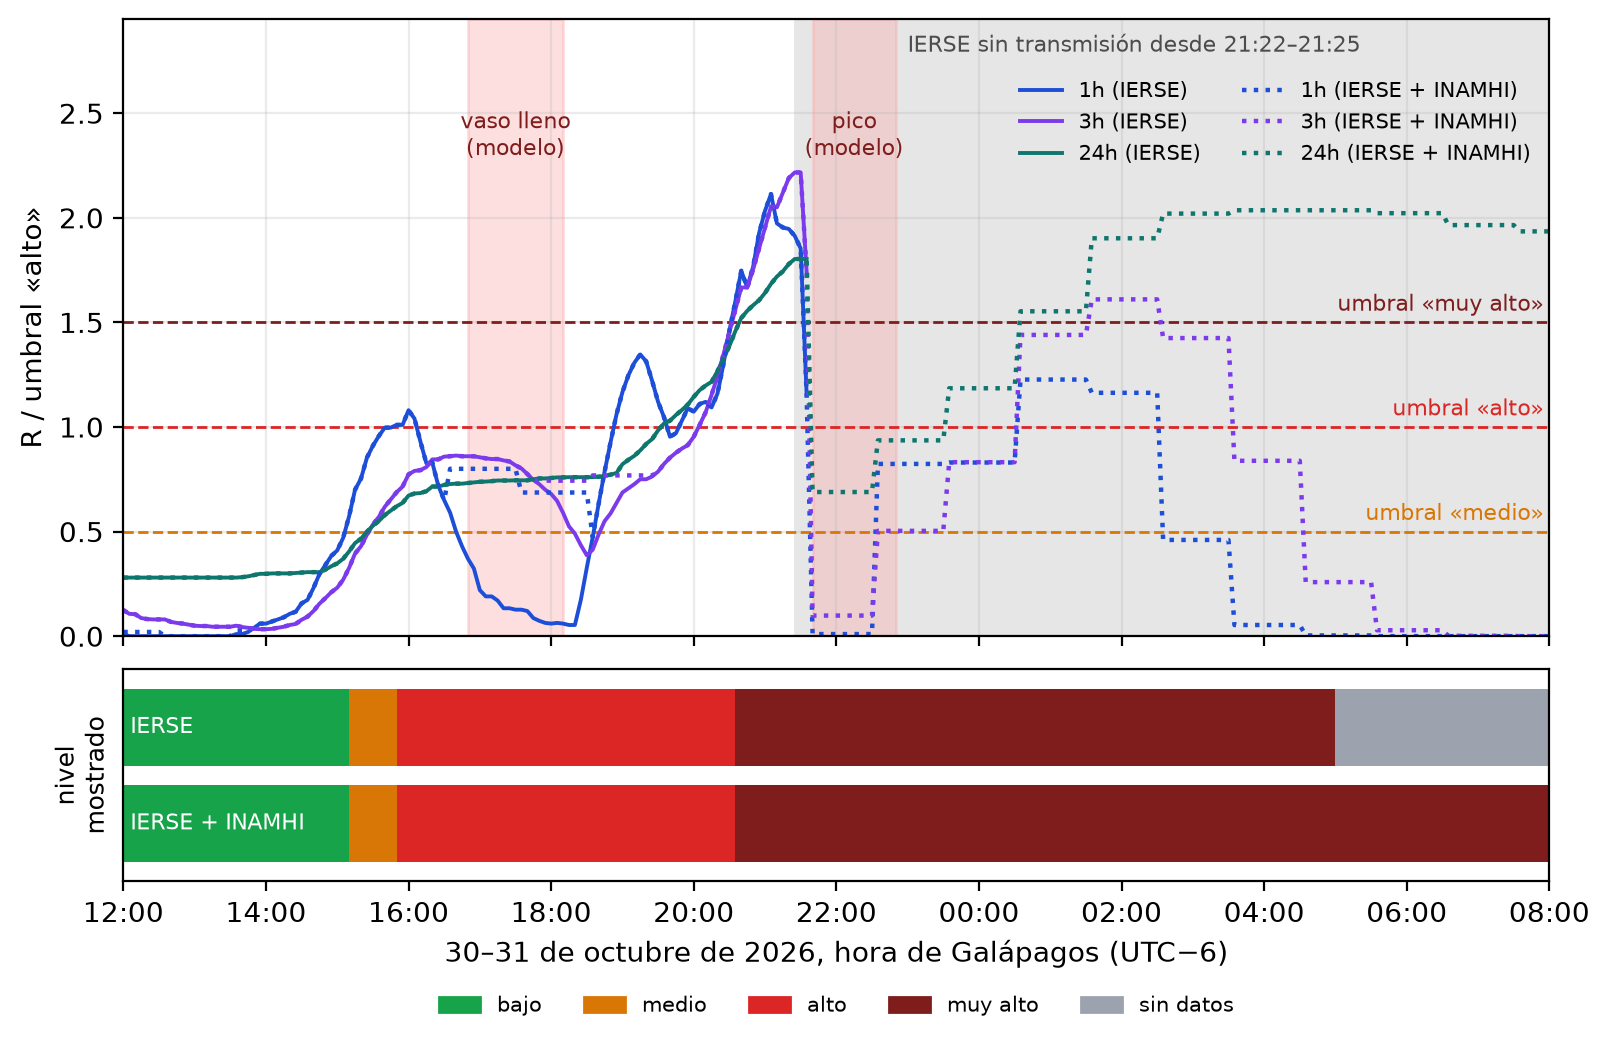
\includegraphics[width=\linewidth]{retro_30oct.png}
  \caption{Prueba retrospectiva de la regla v0.2 en La Cascada, 30--31-oct-2026. Arriba: lluvia de referencia de la zona en 1, 3 y 24~h dividida por el umbral \alto{} de cada ventana (0,5 = medio; 1 = alto; 1,5 = muy alto). Línea continua: solo IERSE (variante A); punteada: IERSE + INAMHI M0191 (B). En rojo claro, el llenado del vaso y el pico de la crecida según el hidrograma modelado; en gris, el corte de transmisión de IERSE. Abajo: nivel mostrado, con persistencia de 8~h y silencio en alerta. Lluvia medida por IERSE-WSN e INAMHI; hitos de modelo propio.}
  \label{fig:retro}
\end{figure}

Las estaciones IERSE dejaron de transmitir a las 21:22--21:25. Desde ahí, las dos variantes divergen:
\begin{itemize}
  \item \textbf{Variante A (solo IERSE).} La zona se queda sin estaciones válidas a las 21:40 y entra la regla de silencio en alerta: el nivel sigue en \enquote{muy alto}. Pasa a \enquote{sin datos} a las 05:00 del 31-oct, 8~h después de la última hora en alerta.
  \item \textbf{Variante B (con INAMHI).} El M0191 sigue transmitiendo, así que la zona conserva una estación válida y la regla de silencio no se activa. A las 21:40 el nivel instantáneo cae a \enquote{medio} y $R_{24}$ baja de 180 a 69~mm, porque las estaciones mudas salen también de la ventana de 24~h. Lo que sostiene el \enquote{muy alto} es la persistencia. Después, la lluvia costera del INAMHI (36,8~mm en una hora y 155~mm en 24~h) devuelve el nivel instantáneo a \alto{} a las 23:35 y a \enquote{muy alto} a las 00:35.
\end{itemize}

En la parte alta, sin el peso de 0,75, Santa Rosa da \alto{} a las 15:20 y \enquote{muy alto} a las 20:00, esta vez por la ventana de 24~h.

La nota de \texttt{clima/docs/umbrales-la-cascada.md} y el panel documentan otra simulación: medio a las 15:15, \alto{} a las 19:05 y muy alto a las 20:55. Esas tres horas se reproducen exactamente si se repone el ajuste en seco de la v0.1 (umbrales $\times 1{,}2$ con $P_{5d} < 36$~mm): con ese ajuste, el primer pulso de Santa Rosa no alcanza el \alto{} en La Cascada ($0{,}75 \times 43 < 36$~mm). Sin él, que es la regla vigente, el \alto{} llega a las 15:50, la misma hora que obtiene el Informe 2026-02 con la lluvia medida \citep{maya2026idf}. Por la misma razón, el argumento con el que la v0.2 quitó el ajuste en seco (\enquote{retrasó la alerta de las 18:51 a las 19:05}) subestima su efecto: sin ajuste, el aviso se adelanta más de tres horas y lo da otra estación.

\subsection{Días de referencia}
La figura~\ref{fig:umbrales} compara los máximos de cada ventana en los tres días de referencia con los umbrales. Los máximos se tomaron evaluando la regla cada 5~min.
\begin{itemize}
  \item \textbf{3-oct.} La regla v0.2 da \enquote{medio} en las dos zonas, con $R_1 = 16$~mm y $R_{24} = 68$~mm. El panel lo presenta como \enquote{bajo}: con ventanas móviles, la hora más lluviosa suma 16~mm, no los 12,6~mm de la hora de reloj.
  \item \textbf{23-oct.} En La Cascada da \enquote{medio}, con 23, 37 y 73~mm en 1, 3 y 24~h. En la parte alta, donde Santa Rosa pesa 1, llega a \alto{} a las 09:00 por la ventana de 24~h: el suelo había pasado a húmedo ($P_{5d} = 54{,}8$~mm), así que el umbral bajó a 80~mm y $R_{24}$ marcaba 83~mm.
  \item \textbf{30-oct.} Supera el \enquote{muy alto} en las tres ventanas.
\end{itemize}

\begin{figure}[t]
  \centering
  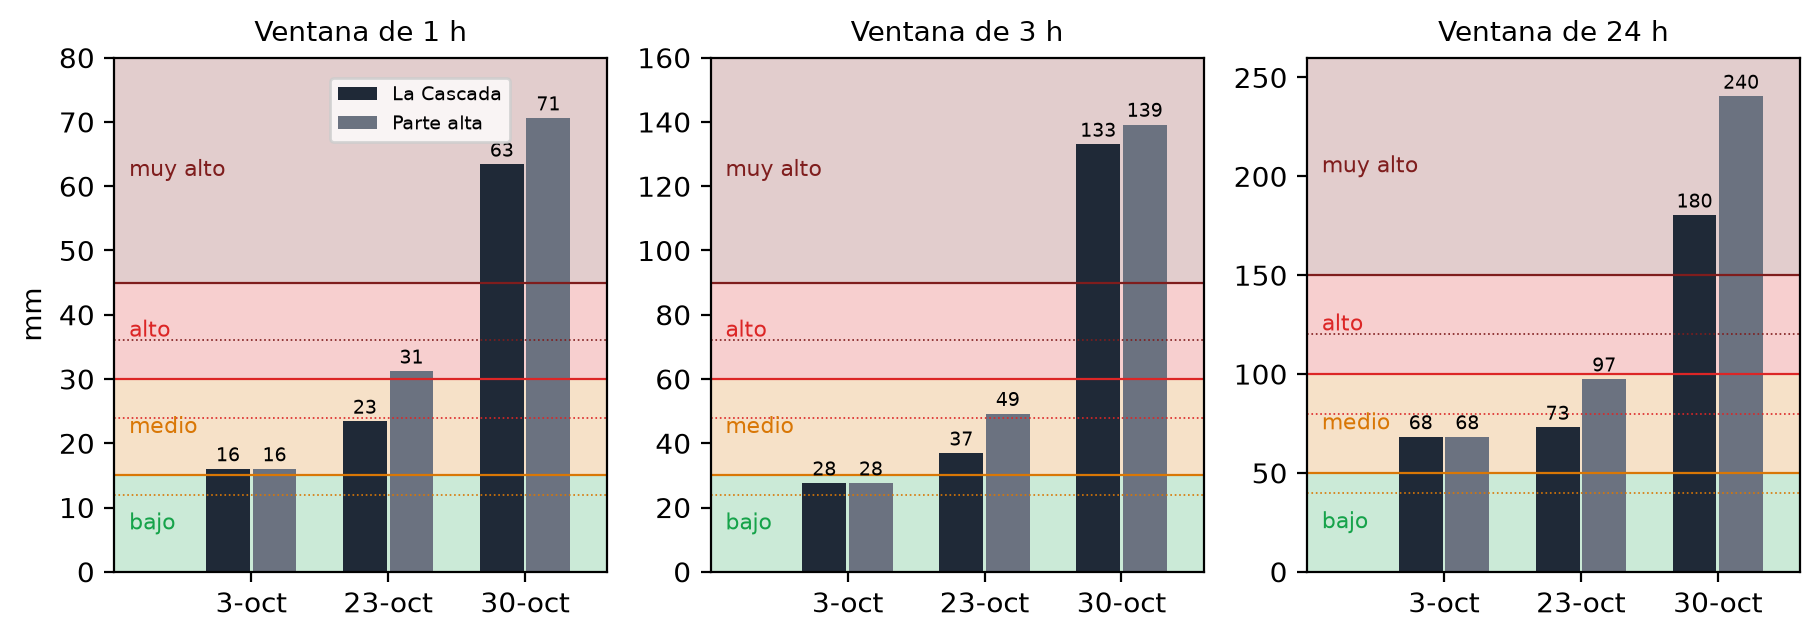
\includegraphics[width=\linewidth]{umbrales_eventos.png}
  \caption{Umbrales de la regla v0.2 por nivel y ventana (líneas continuas; las punteadas son los umbrales con suelo húmedo, $\times 0{,}8$) y máximo de la lluvia de referencia de cada zona en los días de referencia, evaluada cada 5~min con la variante B. En el 3-oct y el 23-oct no consta inundación (sin confirmar, \issue{52}); el 30-oct se inundó La Cascada.}
  \label{fig:umbrales}
\end{figure}

\subsection{El registro completo (abril--noviembre de 2026)}
Entre el 23 de abril y el 2 de noviembre se evaluaron 4651 horas, de las cuales 185 días tuvieron al menos una hora con estaciones válidas (tabla~\ref{tab:registro}). En La Cascada, el nivel mostrado estuvo en \alto{} o más 55 horas, casi todas alrededor del 30-oct.

Fuera de ese evento, la regla dio \alto{} un solo día en La Cascada, el 4-oct, y tres días en la parte alta: el 4-oct, el 23-oct y el 24-oct. Los tres casos tienen el mismo patrón. El \alto{} llega por la ventana de 24~h, con lluvia larga y poco intensa: el 4-oct, $R_{24}$ llegó a 106~mm con un máximo de 7,4~mm en 1~h.

También el \enquote{medio} sale casi siempre de la ventana de 24~h, a veces ayudado por el factor de suelo húmedo. El 14-jun dio \enquote{medio} con 39--65~mm en 24~h y $P_{5d}$ de 54--74~mm. El día siguiente a una lluvia fuerte suele dar \enquote{medio}, porque esa misma lluvia pasa a contar como antecedente. Con suelo seco se clasificaron 128 de los 185 días en La Cascada, 27 con suelo húmedo y 19 en condición normal.

\begin{table}[ht]
  \centering\small
  \caption{Horas en cada nivel con la lluvia medida del 23-abr al 2-nov-2026 (variante B; evaluación al cierre de cada hora). \enquote{Mostrado} incluye la persistencia de 8~h, pero no la regla de silencio. Días por nivel: nivel instantáneo máximo de cada día (UTC$-6$).}
  \label{tab:registro}
  \begin{tabular}{lcccc}
    \toprule
    & \multicolumn{2}{c}{La Cascada} & \multicolumn{2}{c}{Parte alta} \\
    \cmidrule(lr){2-3}\cmidrule(lr){4-5}
    Nivel & Instantáneo & Mostrado & Instantáneo & Mostrado \\
    \midrule
    Bajo & 4184~h & 4236~h & 4156~h & 4200~h \\
    Medio & 73~h & 92~h & 80~h & 111~h \\
    Alto & 11~h & 20~h & 30~h & 46~h \\
    Muy alto & 24~h & 35~h & 2~h & 10~h \\
    Sin datos & 359~h & 268~h & 383~h & 284~h \\
    \midrule
    Días con máximo \enquote{medio} & \multicolumn{2}{c}{6} & \multicolumn{2}{c}{9} \\
    Días con máximo \alto & \multicolumn{2}{c}{2 (4-oct, 1-nov)} & \multicolumn{2}{c}{3 (4, 23 y 24-oct)} \\
    Días con máximo \enquote{muy alto} & \multicolumn{2}{c}{2 (30 y 31-oct)} & \multicolumn{2}{c}{1 (30-oct)} \\
    \bottomrule
  \end{tabular}
\end{table}

Las horas \enquote{sin datos} son muchas: 268 en La Cascada, el 6\,\% del periodo. Se concentran en los cortes de la red IERSE, entre ellos el del 30 al 31-oct, que duró unas 21~h (\issue{62}).

% =====================================================================
\section{Discusión y limitaciones}\label{sec:discusion}

\paragraph{Relación con la evaluación del Informe 2026-02.} El Informe técnico 2026-02 \citep{maya2026idf} propagó 500 tormentas sintéticas por isla con un modelo 2D de inercia local y aplicó la regla v0.2 a seis zonas de impacto, con las estaciones y los pesos de la regla.
\begin{itemize}
  \item La regla avisó a tiempo entre el 87\,\% y el 100\,\% de las inundaciones modeladas, con una anticipación típica de 25~min (Barrio Frío) a 2~h (La Cascada).
  \item Combinada con curvas IDF provisionales, daría \alto{} aproximadamente una vez cada 1,6--1,9 años por zona, lo que equivale a unas 0,4--0,6 falsas alarmas por año y zona.
  \item Con umbrales un 10\,\% más altos, el aviso del 30-oct en La Cascada habría pasado de las 15:50 a las 19:00.
\end{itemize}
Esas cifras son estimaciones de modelo sin validar con inundaciones históricas, pero son la única medida disponible del compromiso entre detección y falsas alarmas. Este informe no las sustituye: el registro medido abarca seis meses y un solo evento con daños. En ese medio año la regla dio en La Cascada un \alto{} sin inundación conocida (4-oct). Es compatible con la frecuencia del Informe 2026-02, pero un semestre no permite estimarla.

\paragraph{El primer aviso del 30-oct vino de la estación equivocada.} El \alto{} de las 15:50 en La Cascada lo provocó Santa Rosa, que está a 6,6~km y no drena hacia el barrio. Llegó una hora antes de que, según el modelo, se llenara el vaso. Si la tormenta hubiera caído solo al oeste, el mismo dato habría dado una falsa alarma en La Cascada. Si hubiera caído solo sobre la cuenca, ninguna estación la habría medido: no hay pluviómetro telemétrico dentro de la cuenca de La Cascada (\issue{19}). El peso de 0,75 suaviza ese efecto, pero no lo resuelve. El Informe 2026-02 identifica un sitio en la cuenca media con mejor capacidad de anticipación que cualquiera de las estaciones actuales.

\paragraph{El vaso se llena antes que cualquier umbral.} Según el modelo, el vaso de La Cascada se llenó entre las 16:50 y las 18:10. Para entonces, la regla solo habría dado \alto{} por Santa Rosa, y con Los Guayabillos no lo habría dado hasta las 18:55. Las viviendas del fondo del vaso se inundan con lluvias moderadas, y una alerta por lluvia no las cubre.

\paragraph{El silencio se juzga por zona, no por estación.} La regla de silencio solo se activa cuando no queda \emph{ninguna} estación válida en la zona. En la variante B, el M0191 costero siguió transmitiendo y la regla no se activó. La salida de las estaciones altas borró además su lluvia de la ventana de 24~h ($R_{24}$ bajó de 180 a 69~mm), y durante unas dos horas el nivel instantáneo fue \enquote{medio}. El \enquote{muy alto} se mantuvo por la persistencia de 8~h, no por la regla de silencio. Con la estación particular WeatherLink en la zona, el efecto sería el mismo. Si el corte hubiera llegado antes del \alto{}, una estación costera viva podría haber mantenido un nivel bajo mientras las estaciones que miden la cuenca callaban.

\paragraph{La ventana de 24~h y el factor de suelo húmedo.} La premisa de la regla es que manda la intensidad en 1--3~h. Sin embargo, fuera del 30-oct todos los \alto{} del registro salen de la ventana de 24~h, con lluvia poco intensa (4-oct: 7,4~mm como máximo en 1~h). El factor de suelo húmedo tiene un efecto parecido. Como $P_{5d}$ excluye las últimas 24~h, la lluvia de un día fuerte pasa a ser antecedente al día siguiente, y los umbrales bajan justo cuando la lluvia ya cesó. Además, $P_{5d}$ se calcula con las estaciones válidas en cada instante: cuando una estación entra o sale, la condición de humedad puede saltar de una hora a otra (el 23-oct pasó de normal a seca y otra vez a normal en dos horas). El Informe 2026-02 trata la humedad antecedente como un parámetro incierto, entre 0 y 100~mm, pero no aísla el efecto del factor.

\paragraph{Calidad de la lluvia medida.} Los pluviómetros de balancín subestiman la lluvia de más de 50~mm/h, que es justo la del 30-oct. El de la estación particular WeatherLink, de 0,254~mm, subestima aún más. Los Guayabillos marca 0~mm desde el 31-oct y Cerro Crocker parece obstruido desde agosto (\issue{56}). La regla del cero solo excluye un pluviómetro obstruido si otra estación de la zona registra 10~mm en 3~h. Las filas horarias de respaldo del INAMHI se guardan a la mitad de la hora, así que adelantan hasta 30~min la lluvia de esa hora. Además, una hora mal convertida entre UTC$-5$ y UTC$-6$ desplazaría todo el aviso una hora; el recolector lo corrige al leer cada fuente.

\paragraph{Calibración y validación.} Los umbrales se fijaron con un evento con daños y dos sin daños conocidos. \enquote{No consta} no significa que no hubo anegamientos: el 3-oct, el 23-oct y el 1--2-nov están por confirmar con el GAD y el COE (\issue{52}). No hay registro de inundaciones con hora y profundidad (\issue{80}). La parte alta y San Cristóbal están sin calibrar, e Isabela no tiene estaciones. La persistencia de 8~h y los hitos del 30-oct salen de modelos propios sin calibrar. Por todo ello, la regla es una herramienta de vigilancia, no un sistema de alerta temprana en el sentido de \citet{basher2006} o de la \citet{wmo2018}. Le faltan el enlace con quien emite la alerta oficial, la difusión y la preparación de la población (\issue{71}).

% =====================================================================
\section{Conclusiones y trabajo futuro}
\begin{enumerate}
  \item La regla v0.2 convierte la lluvia medida en un nivel por zona con cinco elementos: máximo ponderado en 1, 3 y 24~h; umbrales fijos que bajan un 20\,\% con suelo húmedo; persistencia de 8~h; silencio en alerta como alarma; y \enquote{sin datos} en lugar de \enquote{bajo}.
  \item Recalculada con el código del recolector, habría dado \alto{} en La Cascada a las 15:50 del 30-oct y \enquote{muy alto} a las 20:35, entre 5~h y 20~min antes de la llegada modelada del agua al centro del barrio (20:55). El primer aviso lo dio una estación que no drena hacia La Cascada.
  \item En seis meses de registro, fuera del 30-oct, dio \alto{} un día en La Cascada y tres en la parte alta, siempre por la ventana de 24~h con lluvia poco intensa.
  \item El silencio de las estaciones altas no activa la regla de silencio si una estación costera sigue transmitiendo. En ese caso, el nivel lo sostiene solo la persistencia.
  \item Las horas de la simulación publicada en el panel (medio 15:15, alto 19:05, muy alto 20:55) se reproducen solo con el ajuste en seco de la v0.1, que la v0.2 quitó; la regla vigente da \alto{} a las 15:50.
\end{enumerate}

Para pasar de preliminar a calibrada hacen falta:
\begin{itemize}
  \item confirmar si hubo anegamientos el 3-oct, el 23-oct y el 1--2-nov (\issue{52}) y un registro de inundaciones con hora y profundidad (\issue{80});
  \item un pluviómetro telemétrico dentro de la cuenca de La Cascada y en cada poblado (\issue{19}), y la revisión de Cerro Crocker y Los Guayabillos (\issue{56});
  \item recuperar la lluvia de IERSE del corte del 30--31-oct y conocer su causa (\issue{62});
  \item un aviso cuando el recolector deja de correr (\issue{39});
  \item curvas IDF con series locales más largas (\issue{24}, \issue{77}, \issue{78}) y un protocolo de evacuación que use el nivel (\issue{71}).
\end{itemize}

\section*{Disponibilidad de datos y código}
{\small\raggedright El cálculo es reproducible desde el repositorio público \emph{mayait/sosgalapagos-datos}:
\begin{itemize}
  \item regla: \texttt{clima/recolector/inundacion.py} y \texttt{clima/recolector/umbrales\_inundacion.json} (v0.2-preliminar, 2-nov-2026); notas en \texttt{clima/docs/umbrales-la-cascada.md} y \texttt{clima/LEEME.md};
  \item lluvia: \texttt{clima/datos/ierse-wsn/serie\_5min.csv.gz} (UTC$-6$) y \texttt{clima/datos/inamhi/historial/} (UTC$-5$);
  \item primeras superaciones del 30-oct: \texttt{geodatos/scripts/grd\_riesgo\_islas.py}, que escribe \texttt{geodatos/estudios/santa-cruz/\allowbreak datos/riesgo/umbrales\_sat\_30oct.csv}; cronología: \texttt{geodatos/scripts/grd\_linea\_tiempo.py};
  \item prueba retrospectiva y figuras~\ref{fig:retro} y~\ref{fig:umbrales}: \texttt{informes/2026-07-alerta-v02/figuras.py}, que escribe \texttt{figuras/retrospectiva.json}.
\end{itemize}
Los endpoints de las fuentes no se publican. Este informe se compila con \texttt{informes/compilar.sh 2026-07-alerta-v02}.\par}

\bibliographystyle{sosg}
\bibliography{referencias,bib-2026-07}

\end{document}
